\documentclass[10pt]{beamer}
\usepackage[UTF8, noindent]{ctexcap}
% \usefonttheme[onlymath]{serif}
\usetheme{Szeged}
\usecolortheme{beaver}
\usefonttheme{serif}
\usepackage{subfigure}
\usepackage{float}
\usepackage{graphicx, graphics}
\usepackage{float, array, color, ctex}
\usepackage{amsmath, amssymb}
\usepackage{multicol, multirow, makecell, tabu, dcolumn}
\usepackage{fancyhdr, lastpage}
\usepackage{listings, xcolor}
\usepackage{enumerate}
\usepackage{xeCJKfntef}
\usepackage{fontspec, xunicode, xltxtra}
\usepackage{setspace}
\usepackage{geometry}
% ================================================================
\title{论文选题\&前段时间总结}
\date{\today}% 可以输入\today \zhtoday 或者直接手打
\author{张锦羽}
\institute{西安交通大学管理学院} %学院、大学、单位等
\usepackage{color}
\definecolor{dkgreen}{rgb}{0,0.6,0}
\definecolor{gray}{rgb}{0.5,0.5,0.5}
\definecolor{mauve}{rgb}{0.58,0,0.82}
% \usepackage{pgfpages}

% \setbeameroption{hide notes}
% \setbeameroption{show notes on second screen=right}

% \usetheme{quito-light}
\usetheme{CambridgeUS}
\footnotesize
\begin{document}
%_____________________________________________________
% Title page
% \frame[plain]{
% \titlepage
% }
\begin{frame}
\titlepage
    
\end{frame}
%_____________________________________________________
% ======================{目录页}===========================
% 左右分栏选这页
\begin{frame}{目录}
    \tableofcontents 
\end{frame}
\section{目前工作进展}
\begin{frame}[plain]{猫途鹰网站爬虫}
    %两侧分栏
    \begin{columns}
        \column{0.5\textwidth}
        \begin{figure}
            \centering
            \subfigure{
            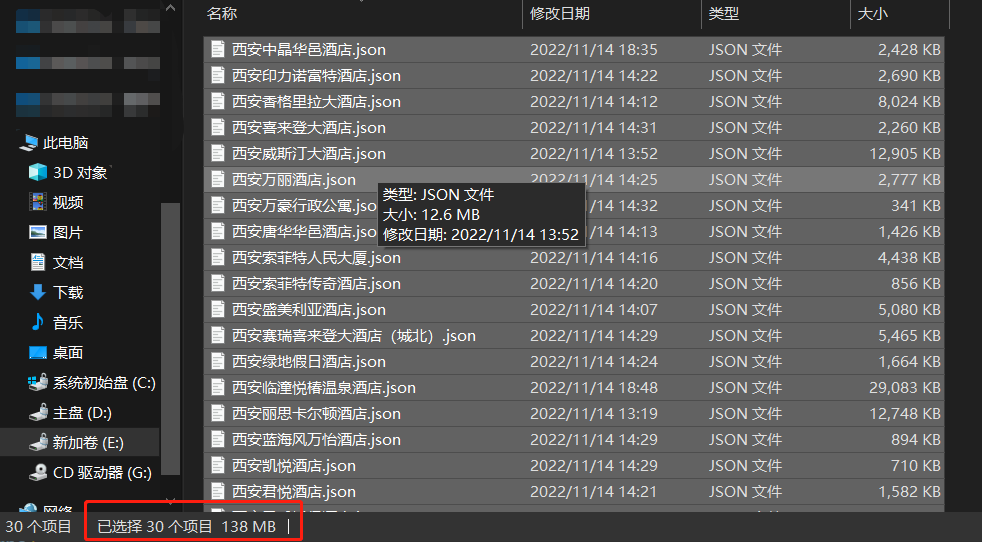
\includegraphics[width=1\textwidth]{figures/爬的json.png}}
            \subfigure{
        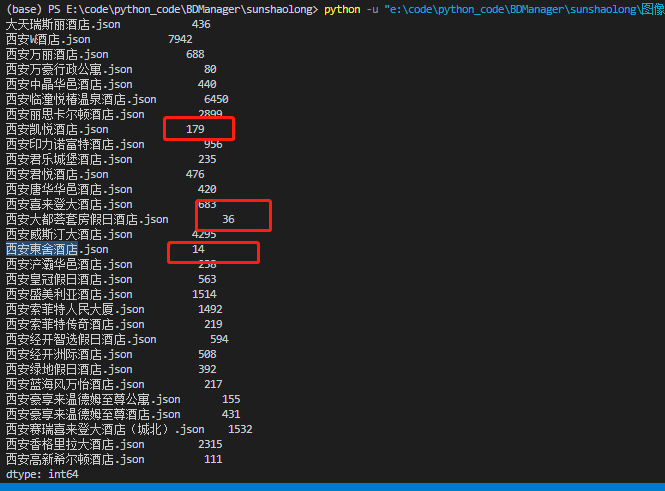
\includegraphics[width=1\textwidth]{figures/爬的数量.png}}
    \end{figure}
        \column{0.5\textwidth}
        \begin{figure}[ht]
            \centering
            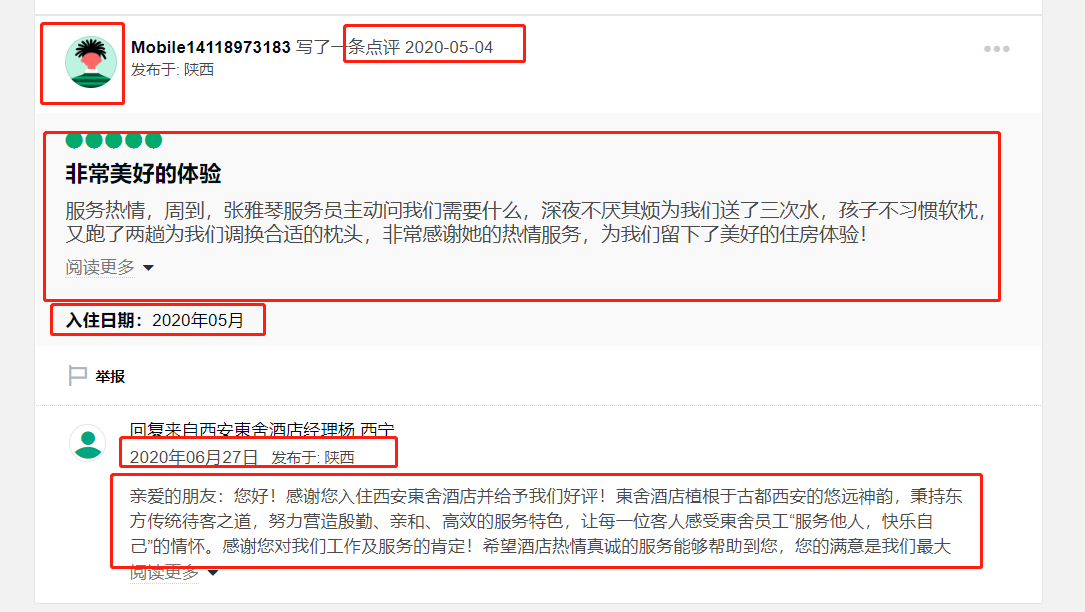
\includegraphics[width=0.9\textwidth]{figures/详细信息.png}
        \end{figure}
        
        \footnotesize{我基本上把能获取到的信息全爬下来了,而且猫途鹰网获取数据非常方便,我找到了接口,可以直接下载json数据,根据论文需要我还可以获取更多的数据。
                \begin{enumerate}
                    \item 用户回复文本内容、用户回复时间、用户注册时间、用户附的照片、用户的评价星级(对酒店的打分)、用户出行方式、用户的入住时间、用户评论发布时间
                    ....
                    \item {\color{red}酒店经纬度}、酒店回复内容、酒店照片、酒店回复时间
                    \item {\color{red}景点的经纬度、评论还有美食的经纬度、评论}
                \end{enumerate}}
    \end{columns}
\end{frame}
% ========================={ppt无标题版}=========================
\begin{frame}
    发现几个有意思的地方:用户评论中都是包含有一个标题属性的:
    \begin{figure}
        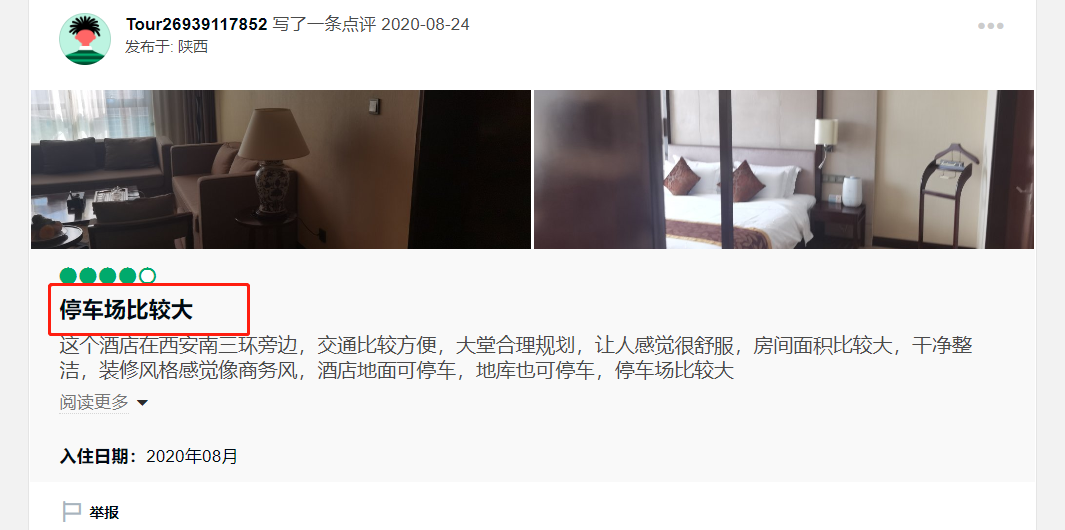
\includegraphics[width=1\textwidth]{figures/评论标题.png}
    \end{figure}
    标题可能是下面评论的概括,也可以是评论信息中用户最想突出的部分。能否通过评论标题预测用户的打分倾向?
\end{frame}
% ========================={ppt无标题版}=========================
\begin{frame}
    \begin{columns}
        \begin{column}{0.5\textwidth}
            \begin{figure}
                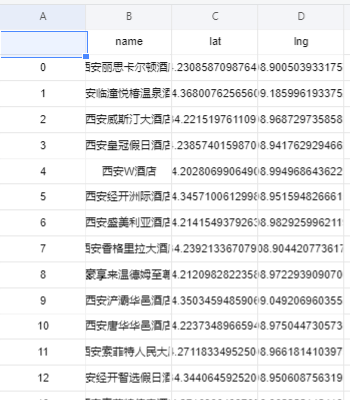
\includegraphics[width=1\textwidth]{figures/酒店经纬度.png}
            \end{figure}
        \end{column}
        \begin{column}{0.5\textwidth}
            酒店,景点,美食,三者的经纬度和评论都可以获取。是否可以作出一些东西呢?{\color{red}(以前打数模的时候做过西安市房价预测的题目,当时就是爬取了一些二手房信息利用百度地图api可视化出来)}
            \begin{itemize}
                \item 由于一部分用户可能只是偶尔使用该平台,但是可能有一些用户是该平台的深度用户。使用全部用户评论对酒店进行评价时,需要不需要考虑不同类别用户之间的权重?
                \item 有些用户注册比较早,有些用户注册晚,注册时间会不会对两种用户有影响(比如同一用户分为后疫情和前疫情去研究?但是如何控制变量得到疫情影响的因果效应?)
            \end{itemize}
        \end{column}
    \end{columns}
\end{frame}
% ========================={ppt无标题版}=========================
\begin{frame}
    我想做的方向是偏向统计学+机器学习方法+实证方法做出一篇文章,对标的期刊应该是\textbf{运筹与管理、管理工程学报}。
    
    该文章的大概流程应该是:引言,综述,实验部分(数据获取、数据探索、特征工程:\textbf{机器学习方法}),实证部分(探究政策,时间,地理等因素,某变量对某变量的影响),管理学意义。
    \begin{figure}[H]
        \subfigure{
        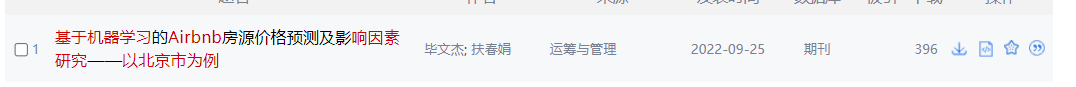
\includegraphics[width=1\textwidth]{figures/运筹与管理.png}
        }
        \subfigure{
            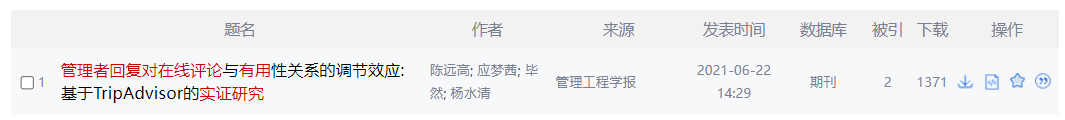
\includegraphics[width=1\textwidth]{figures/管理工程学报.png}
        }
    \end{figure}
    \begin{columns}
        \column{0.5\textwidth}
        \begin{itemize}
            \item 做评论中文本和图片相关的实证分析。但是我题目没想好,第一篇论文感觉自己把握不好,选题太大或者太小没概念。而且太小了感觉又太简单没什么意义...
        \end{itemize}
            
        \column{0.5\textwidth}
        \begin{itemize}
            \item 我发现可以爬到一些空间的数据,而且可以爬到西安市top排名的酒店和top排名的景点。我觉得很有意思,可以和老师讨论一下。如果能做运筹与优化方面的我也挺感兴趣的。
        \end{itemize}
    \end{columns}
\end{frame}


\section{《中国旅游大数据研究:...》论文阅读}%这些标题最后会归入目录中
%============================{block}=================================
\begin{frame}{\normalsize{中国旅游大数据研究:二十年回顾与展望}}
    \par 本文是类似于综述的一篇文章,回顾了中国旅游大数据发展的20年来,知网上核心期刊的发刊数量以及研究领域等。文章根据旅游大数据中数据类型的不同,分为了不同的研究方法,我在阅读这篇文章的过程中联系了我的研究问题,将注意力重点关注到了UGC数据的研究方法中。
\end{frame}
%============================{block}=================================
\begin{frame}{\normalsize{中国旅游大数据研究:二十年回顾与展望}}
\small{本文中将旅游大数据的数据类型分为了三类:UGC(User Generated Content)数据、设备数据(GPS、气象、智能穿戴设备)、事务性数据(网页搜索、网页浏览、在线预定数据)。

根据获取难度,UGC数据是最容易获取的,设备数据和事务性数据一般是私密的,难以获取的。
\begin{columns}
    \begin{column}{0.5\textwidth}
        旅游大数据UGC研究数据:
        \begin{figure}
            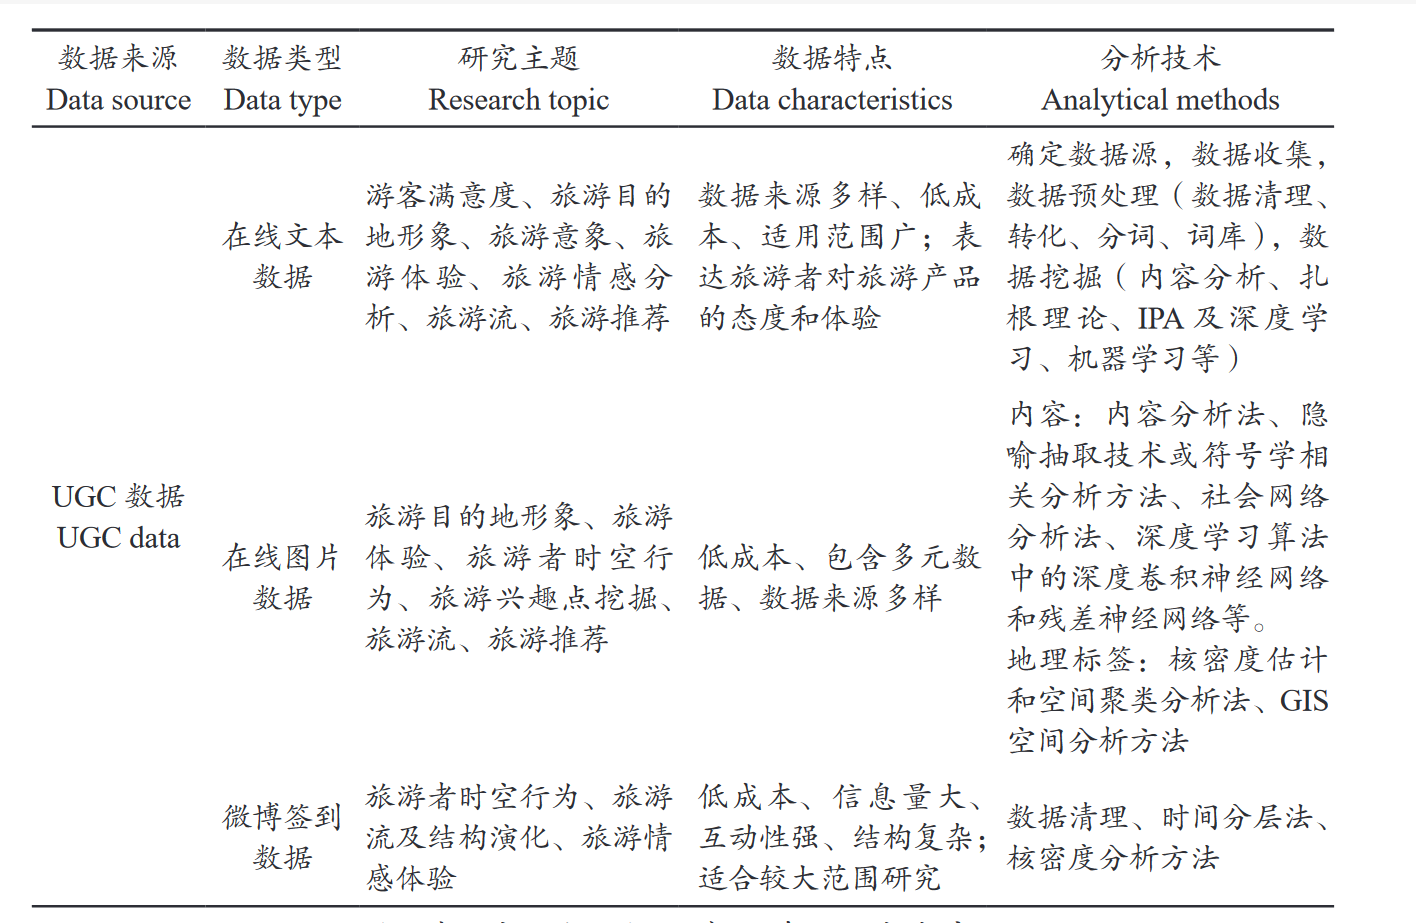
\includegraphics[width=1\textwidth]{figures/UGC数据研究方法.png}
        \end{figure}
    \end{column}
    \begin{column}{0.5\textwidth}
        我获取到的主要是UGC(User Generated Content)数据(用户在线评论、用户配图、用户评分等)。此外还有一些事务型数据:如开源的百度指数api可以调用。
        \begin{itemize}
            \item \textbf{文本数据的处理流程:}\\数据清洗,去重去空$\Longleftrightarrow$数据转化,同义词$\Longleftrightarrow$分词,词向量化$\Longleftrightarrow$评论分类,情感分析等
            \item \textbf{图片数据的处理流程:}
            \\内容分析法、cv和图像处理辅助图片内容 识别及分类。\\图片地理空间分析(拍摄图片的位置、时间等主要是一些图片分享的网站有相关的接口,tripadvisor无此类接口)。
        \end{itemize}
    \end{column}
\end{columns}}
\end{frame}
%============================{block}=================================
\section{总结}
\begin{frame}{科研任务总结}
    \begin{block}{总结}
        \begin{enumerate}
            \item 确定了猫途鹰爬虫的难度不大,数据获取非常容易。探索了一些能够获取到的数据类型。基本上平台上有的都能获取到,非常方便。
            \item 选择了一些重点的数据进行思考:评论中包含标题信息和图片信息,也有用户评星。研究影响用户评价的因素?个体异质性?是否可以找到一些明星用户,比较他们对于不同酒店的评价,缓解个体异质性。给酒店管理决策?
            \item 用户id与酒店id?我可以获取到一个用户所有的评论数据。可以根据评论的时间和地点知道用户的活动轨迹。是否可以依据一些明星用户的轨迹做研究。(定义明星用户,半年内评论超过xx次的)
            \item 图片数据不知道怎么处理....我对cv还是小白,但简单操作或者调包跑模型应该不在话下的,这方面我学的很快,只要有明确的方向。
            \item ....
        \end{enumerate}
    \end{block}
\end{frame}
\end{document}
